%=====================================================================
%  Master's Thesis Defense — Banking & Quantitative Finance
%  "Statistical Properties of the Sharpe Ratio Estimator"
%  Beamer + Metropolis.  Compile with XeLaTeX or LuaLaTeX for the
%  intended Fira Sans look; pdfLaTeX also works (default fonts).
%  Run the engine twice so the progress bars / section pages resolve.
%=====================================================================
\documentclass[aspectratio=169,10pt]{beamer}
\usetheme{metropolis}

\usepackage{booktabs}
\usepackage{amsmath,amssymb}
\usepackage{graphicx}
\usepackage{xcolor}
\usepackage{subcaption}   % subfigure grid on the bias-correction slide
% \usepackage[scale=2]{ccicons}   % optional (not required)

% --- Bibliography for the citation footnotes on the "Prior work" slide -------
% The markers a–d there use \parencite, which needs biblatex + a references.bib
% holding the keys Lo2002, Mertens2002, Lopez2025, Lopez2026.
% If you \input this deck into a thesis file that ALREADY loads biblatex,
% delete these two lines (the master file's setup takes over).
\usepackage[style=authoryear,backend=biber]{biblatex}
\addbibresource{biblio.bib}

% --- Academic accent: deep-blue frame titles + red alert for emphasis
\definecolor{accentblue}{HTML}{1F4E79}
\definecolor{alertred}{HTML}{C0392B}
\setbeamercolor{frametitle}{bg=accentblue,fg=white}
\setbeamercolor{alerted text}{fg=alertred}

\metroset{progressbar=frametitle, sectionpage=progressbar, block=fill}

% Slightly tighter list spacing for content-dense slides
\setbeamertemplate{itemize items}[circle]

\title{Statistical Properties of the Sharpe Ratio Estimator}
\subtitle{A Robustness Analysis under Various Assumptions on Returns}
\author{Fabrizio Ortega Suni}
\institute{Master’s Thesis in Banking and Quantitative Finance \\
           Supervisor: Manuel Ángel Domínguez Toribio}
\date{May 2026}
% \titlegraphic{\hfill\includegraphics[height=1.2cm]{figures/logo.pdf}}

\begin{document}

\maketitle

%=====================================================================
\section{How much can you trust a Sharpe ratio?}
%=====================================================================

% ---------- SLIDE 1 — Hook ----------
\begin{frame}{How reliable is this number?}
  \begin{columns}[T]
    \begin{column}{0.40\textwidth}
      \begin{itemize}
        \item A reported Sharpe ratio of \alert{$\widehat{\mathrm{SR}} = 0.5$}.
        \item A population quantity, estimated from a finite sample:
              \[ \mathrm{SR} = \frac{\mu}{\sigma}, \qquad
                 \widehat{\mathrm{SR}} = \frac{\hat\mu}{\hat\sigma} \]
        \item One question for the whole talk: \textbf{how much should we trust it?}
      \end{itemize}
    \end{column}
    \begin{column}{0.60\textwidth}
      \centering
      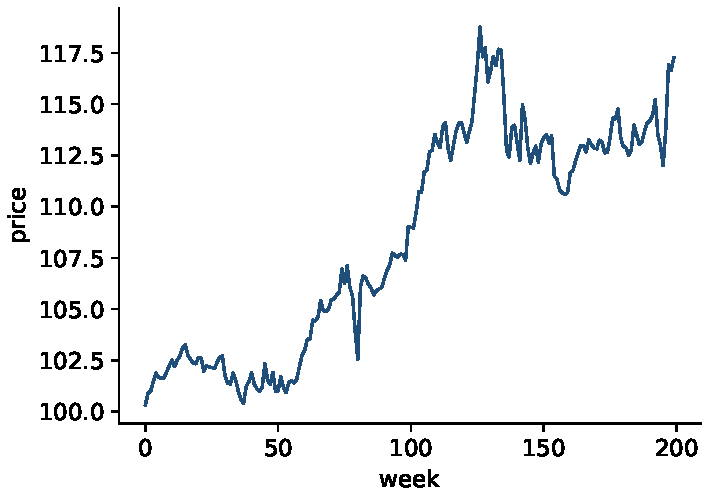
\includegraphics[width=\linewidth]{figures/price_hook.pdf}\\[2pt]
      {\footnotesize Reported $\widehat{\mathrm{SR}}=0.5$.}
    \end{column}
  \end{columns}
\end{frame}

% ---------- SLIDE 2 — Asymptotic variance ----------
\begin{frame}{Measuring reliability: the asymptotic variance}
  \[ \sqrt{T}\,\bigl(\widehat{\mathrm{SR}}-\mathrm{SR}\bigr)
     \;\xrightarrow{\,d\,}\; \mathcal{N}\!\bigl(0,\; V_{\widehat{\mathrm{SR}}}\bigr) \]

  \small
  Classical IID--Normal result (Lo, 2002):\quad
  $\displaystyle V_{\widehat{\mathrm{SR}}}^{\,\mathrm{IID\,N}} = 1 + \tfrac{1}{2}\,\mathrm{SR}^2$
  \hfill
  CI:\quad
  $\displaystyle \mathrm{IC}_{1-\alpha}
     = \Bigl[\, \widehat{\mathrm{SR}} \pm z_{1-\alpha/2}\sqrt{V_{\widehat{\mathrm{SR}}}/T} \,\Bigr]$
  \normalsize

  \vspace{0.4em}
  \begin{columns}[c]
    \begin{column}{0.5\textwidth}\centering
      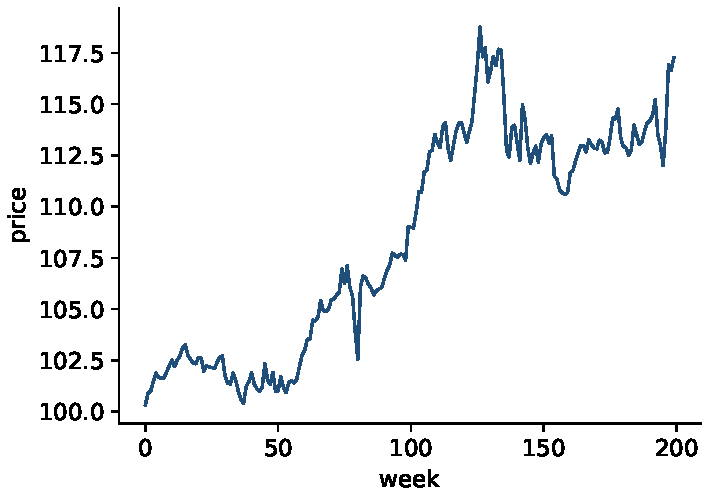
\includegraphics[width=\linewidth,height=3cm,keepaspectratio]{figures/price_hook.pdf}
    \end{column}
    \begin{column}{0.5\textwidth}\centering
      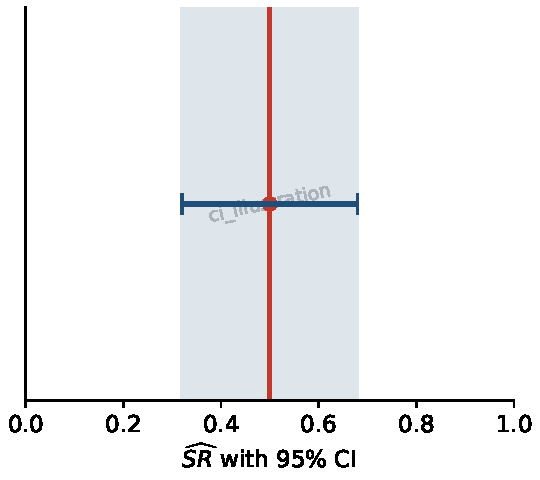
\includegraphics[width=\linewidth,height=3cm,keepaspectratio]{figures/ci_illustration.pdf}
    \end{column}
  \end{columns}

  \vspace{0.3em}
  {\footnotesize All of this rests on the IID--Normal assumption.}
\end{frame}

% ---------- SLIDE 3 — Stylized facts ----------
\begin{frame}{Real returns are not IID Normal --- Cont's stylized facts}
  \centering
  \begin{columns}[T]
    \begin{column}{0.5\textwidth}\centering
      {\small Heavy tails}\\[1pt]
      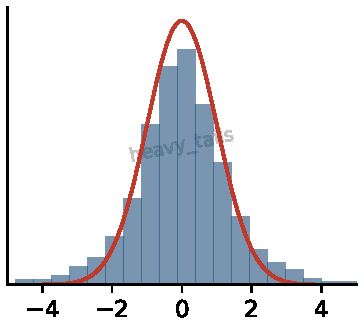
\includegraphics[height=2.5cm,keepaspectratio]{figures/heavy_tails.pdf}\\[3pt]
      {\small Volatility clustering}\\[1pt]
      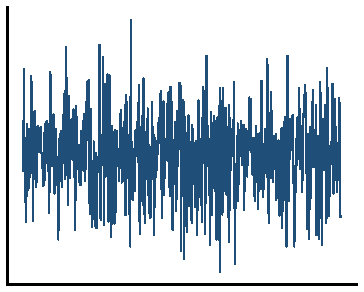
\includegraphics[height=2.5cm,keepaspectratio]{figures/vol_clustering.pdf}
    \end{column}
    \begin{column}{0.5\textwidth}\centering
      {\small Skewness}\\[1pt]
      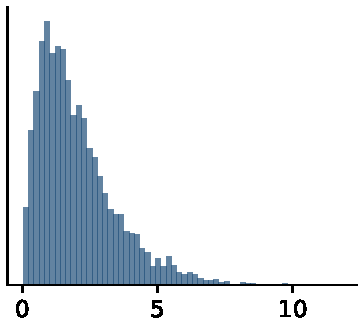
\includegraphics[height=2.5cm,keepaspectratio]{figures/skewness.pdf}\\[3pt]
      {\small Autocorrelation (low freq.)}\\[1pt]
      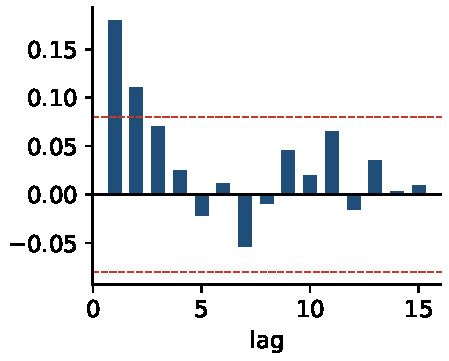
\includegraphics[height=2.5cm,keepaspectratio]{figures/autocorrelation.pdf}
    \end{column}
  \end{columns}
  \vspace{0.35em}
  {\footnotesize Each breaks an assumption behind $1+\tfrac12\mathrm{SR}^2$.}
\end{frame}

% ---------- SLIDE 4 — Prior work ----------
\begin{frame}{Prior work: one variance formula per model}
  \centering
  \footnotesize
  \begin{tabular}{@{}ll@{}}
    \toprule
    Model & $V_{\widehat{SR}}$ \\
    \midrule
    IID Normal\textsuperscript{a}       & $1 + \frac{1}{2}SR^2$ \\[4pt]
    IID Non-Normal\textsuperscript{b}   & $1 - \gamma\,SR + \tfrac{\kappa-1}{4}SR^2$ \\[4pt]
    AR(1)\textsuperscript{c}            & $\frac{1+\phi}{1-\phi} - \frac{1 + \phi +\phi^2}{1 - \phi^2}\gamma SR + \frac{1+\phi^2}{1-\phi^2} \frac{\kappa - 1}{4}SR^2$ \\[8pt]
    GARCH(1,1)\textsuperscript{d}       & $1 - \frac{1-\beta}{1-\alpha-\beta}\gamma SR + \frac{\kappa-1}{4}\frac{(1-\beta)^2 (1+\alpha+\beta)}{(1-\alpha-\beta)(1-2\alpha\beta-\beta^2)}SR^2$ \\
    \bottomrule
  \end{tabular}

  \normalsize
  \vspace{0.7em}
  \alert{The point estimate $\widehat{\mathrm{SR}}$ is identical in every row}
  --- only the variance (interval width) changes.

  \vfill
  {\scriptsize $\gamma=$ skewness, \quad $\kappa=$ kurtosis.}

  \vspace{0.3em}
  {\scriptsize\raggedright
   \textsuperscript{a}\,\parencite{Lo2002}\quad
   \textsuperscript{b}\,\parencite{Mertens2002}\quad
   \textsuperscript{c}\,\parencite{Lopez2025}\quad
   \textsuperscript{d}\,\parencite{Lopez2026}\par}
\end{frame}

% ---------- SLIDE 5 — Contribution ----------
\begin{frame}{Contribution: closing the gap --- AR(1)-GARCH(1,1)}
  \footnotesize
  \setlength{\parskip}{0pt}%
  \setlength{\abovedisplayskip}{2pt}\setlength{\belowdisplayskip}{2pt}%
  \setlength{\abovedisplayshortskip}{1pt}\setlength{\belowdisplayshortskip}{1pt}%
  No closed form existed when \alert{both} features are present:
  AR in the mean \textbf{and} GARCH in the variance.

  \vspace{0.4em}
  \begin{block}{Asymptotic variance, AR(1)-GARCH(1,1), general innovations}
    \[
      \resizebox{\textwidth}{!}{$\displaystyle
      V_{\widehat{\mathrm{SR}}}=\frac{1+\phi}{1-\phi}
        -\,\frac{(1+\phi+\phi^{2})}
                {(1-\phi^{2})(1+2\phi\alpha-\phi\beta)}
           \left[\,2\phi\alpha
             +\frac{(1-\beta)\bigl(1-\phi(\alpha+\beta)\bigr)}{1-\alpha-\beta}\,\right]\,\gamma\,\mathrm{SR}
        +\frac{1}{4(1-\phi^{2})}
         \left(4\phi^{2}+((1+\phi^2)\kappa -1-5\phi^2)\frac{\Sigma}{1+X}
               +\gamma^{2}Z\Bigl(N-\frac{M}{1+X}\Sigma\Bigr)\right)\mathrm{SR}^{2}$}
    \]
  \end{block}

  \vspace{0.1em}
  {\scriptsize $\gamma=$ skewness, \quad $\kappa=$ kurtosis.}
  
  \vfill
  \textbf{Auxiliary terms:}
  \[
    M = 1+\phi^{2}(2\alpha-\beta),\qquad
    N = 2\phi^{2}\alpha+\frac{1-\beta}{1-\alpha-\beta}\bigl(1-\phi^{2}(\alpha+\beta)\bigr),\qquad
    X = \alpha\frac{6\phi^2}{1-\phi^{2}(\alpha+\beta)}\frac{1-\alpha\beta-\beta^2}{1-2\alpha\beta-\beta^2}
  \]
  \[
    \Sigma = \tfrac{2}{3}X
             +\frac{(1-\beta)^{2}}{(1-\alpha-\beta)^{2}}\,
              \frac{1-(\alpha+\beta)^{2}}{1-2\alpha\beta-\beta^{2}},\qquad
    Z = \tfrac{3}{2}\alpha\,
        \frac{(1-\phi(\alpha+\beta))(1+\phi+\phi^{2})^{2}}
             {(1+\phi)^{2}(1+2\phi\alpha-\phi\beta)^{2}}\,
        \frac{4\phi}{1-\phi^{2}(\alpha+\beta)}
  \]

  
  
\end{frame}


% ---------- SLIDE 6 — Sensitivity ----------
\begin{frame}{Which parameters move the variance?}
  \begin{columns}[c]
    \begin{column}{0.5\textwidth}\centering
      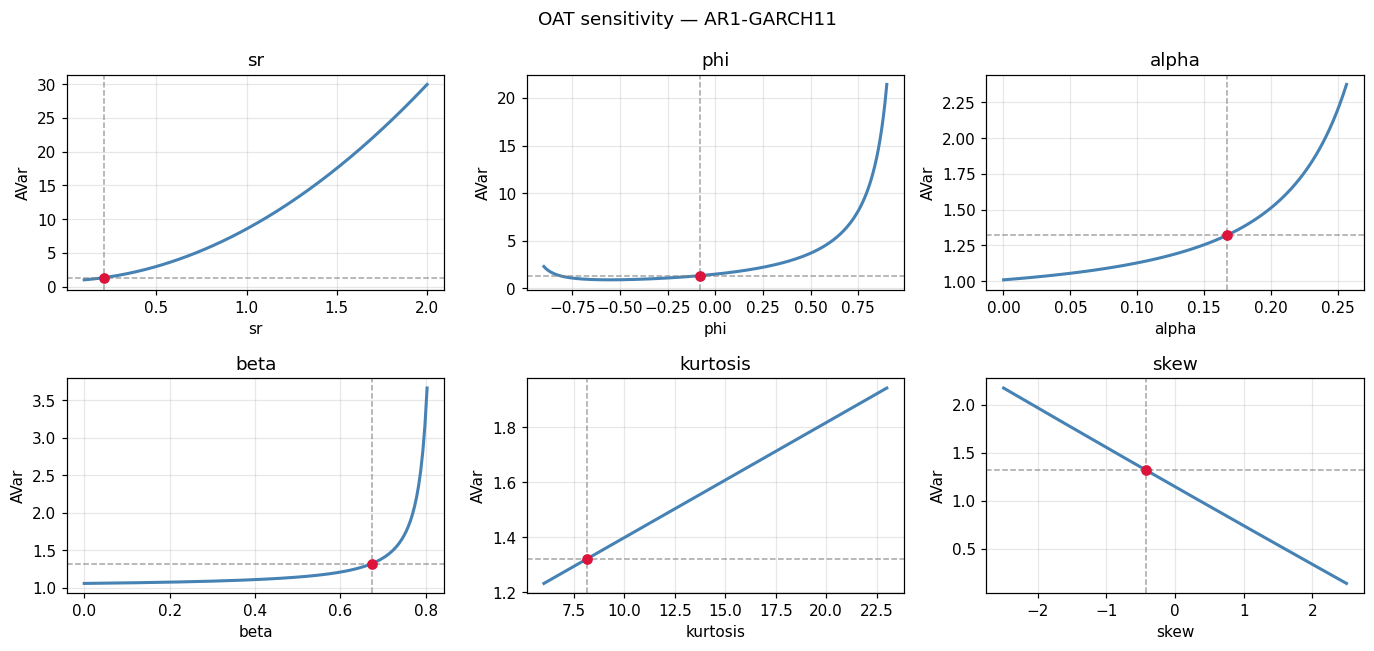
\includegraphics[width=\linewidth,height=4.3cm,keepaspectratio]{figures/oat_sweeps.png}\\
      {\footnotesize One-at-a-time sweep}
    \end{column}
    \begin{column}{0.5\textwidth}\centering
      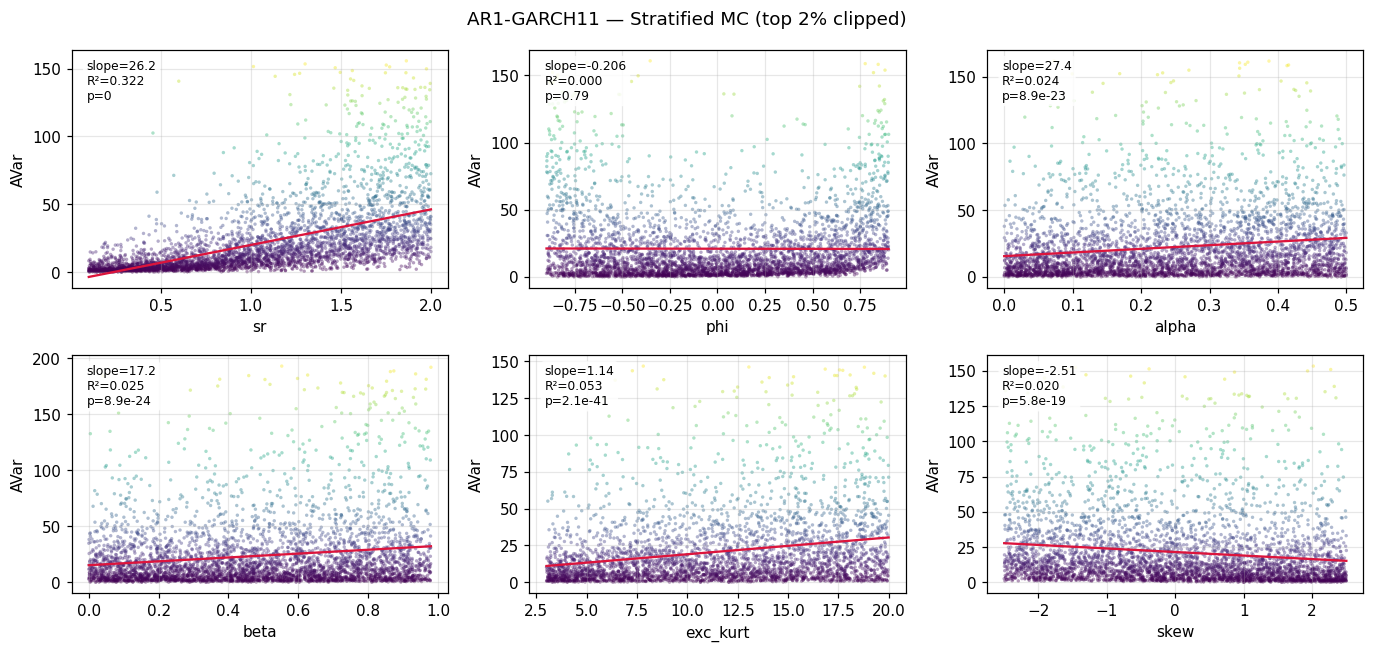
\includegraphics[width=\linewidth,height=4.3cm,keepaspectratio]{figures/mc_scatter.png}\\
      {\footnotesize Axis-stratified Monte Carlo}
    \end{column}
  \end{columns}
  \vspace{0.4em}
  \begin{itemize}
    \item \alert{SR is the dominant driver} (convex, quadratic).
    \item Kurtosis \& skewness next (steady, $\sim$linear).
    \item $\phi,\alpha,\beta$: mild on average, \textbf{explosive near the boundaries}
          ($\phi\to1$, $\alpha+\beta\to1$).
  \end{itemize}
\end{frame}

%=====================================================================
\section{Do the confidence intervals actually work?}
%=====================================================================

% ---------- SLIDE 7 — Why coverage ----------
\begin{frame}{Testing the intervals: coverage on synthetic data}
  Simulate from a known DGP; measure how often the 95\% interval contains
  the true SR.

  \vspace{0.6em}
  Why coverage, not variance?
  \begin{itemize}
    \item It is the \textbf{inferential target} the user cares about.
    \item It is a \textbf{joint test} --- catches bad variance, bias, \emph{and} non-normality.
    \item It has a \textbf{calibrated target}: a binomial acceptance band around $0.95$.
  \end{itemize}

  \vspace{0.4em}
  {\footnotesize Curve below the band $\Rightarrow$ intervals too narrow
  $\Rightarrow$ overconfident.}
\end{frame}

% ---------- SLIDE 8 — Coverage, core result ----------
\begin{frame}{Two findings: sign asymmetry \& the AR-GARCH gap}
  \begin{columns}[c]
    \begin{column}{0.5\textwidth}\centering
      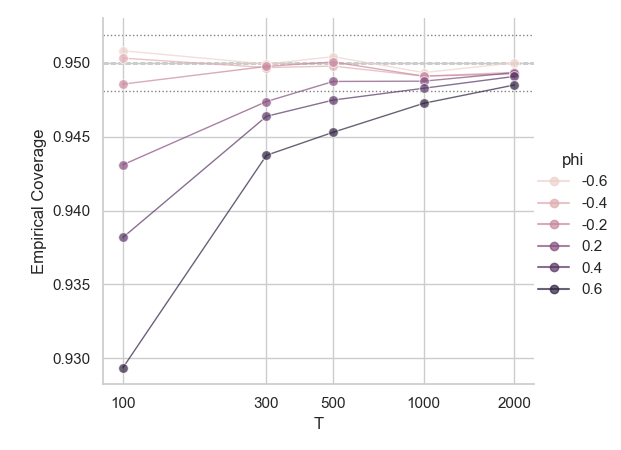
\includegraphics[width=\linewidth,height=4.2cm,keepaspectratio]{figures/phi_line.png}\\
      {\footnotesize AR(1) DGP: $\rho=+0.6$ vs $\rho=-0.6$}
    \end{column}
    \begin{column}{0.5\textwidth}\centering
      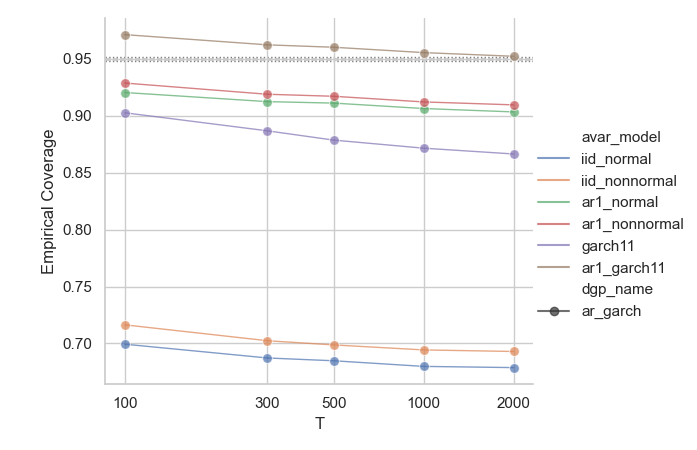
\includegraphics[width=\linewidth,height=4.2cm,keepaspectratio]{figures/serial_hetero_line.png}\\
      {\footnotesize AR-GARCH DGP: all candidate models}
    \end{column}
  \end{columns}
  \vspace{0.3em}
  \pause
  \begin{itemize}
    \item Autocorrelation is \alert{asymmetric in sign}: positive $\rho \Rightarrow$
          coverage $\approx \alert{0.69}$; negative $\rho \Rightarrow \approx \alert{0.99}$.
    \item With both stylized facts present,
          \alert{only the AR-GARCH formula closes the gap}.
  \end{itemize}
\end{frame}

% ---------- SLIDE 9 — Coverage at the edges ----------
\begin{frame}{Where the asymptotics strain}
  \begin{columns}[c]
    \begin{column}{0.5\textwidth}\centering
      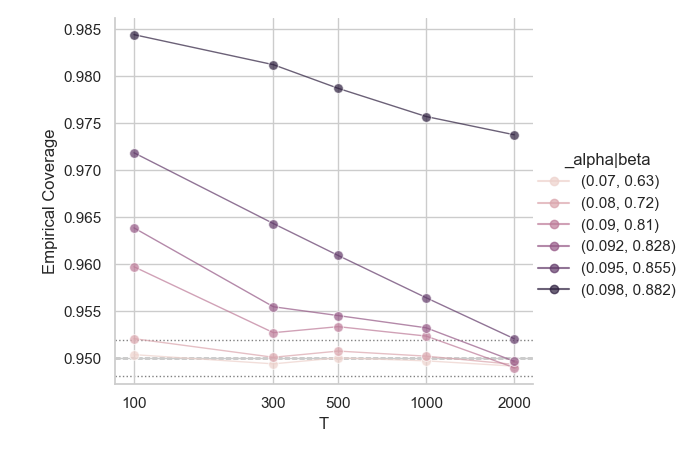
\includegraphics[width=\linewidth,height=4.2cm,keepaspectratio]{figures/a_plus_b_line.png}\\
      {\footnotesize GARCH persistence $\alpha+\beta$}
    \end{column}
    \begin{column}{0.5\textwidth}\centering
      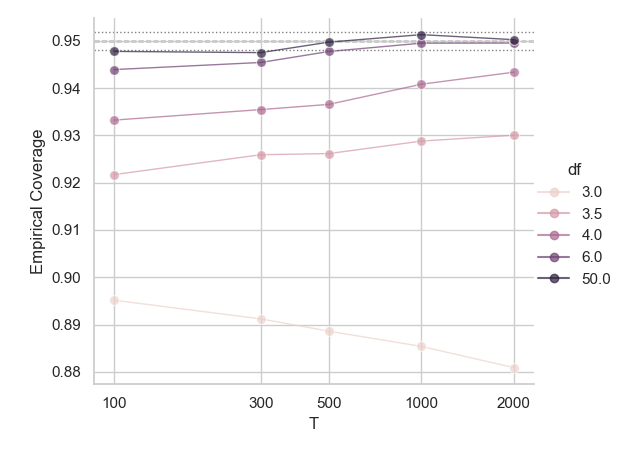
\includegraphics[width=\linewidth,height=4.2cm,keepaspectratio]{figures/slow_conv_line.png}\\
      {\footnotesize Student-$t$ degrees of freedom $df$}
    \end{column}
  \end{columns}
  \vspace{0.3em}
  \begin{itemize}
    \item Higher GARCH persistence $\Rightarrow$ \textbf{slower} convergence to nominal.
    \item \alert{No fourth moment} ($df<4$): coverage \textbf{drifts away} as $T$ grows.
    \item Matches Kao et al.\ (2025): rate $T^{\,\varphi}$ with
          $\varphi=1-2/\kappa<\tfrac12$ --- $\sqrt{T}$ breaks down.
  \end{itemize}
\end{frame}

%=====================================================================
\section{Is the point estimate even right?}
%=====================================================================

% ---------- SLIDE 10 — Bias & the Christie error ----------
\begin{frame}{The point estimate is biased --- and a popular fix is wrong}
  \setlength{\abovedisplayskip}{3pt}\setlength{\belowdisplayskip}{3pt}%
  \setlength{\abovedisplayshortskip}{1pt}\setlength{\belowdisplayshortskip}{1pt}%
  $\widehat{\mathrm{SR}}=\hat\mu/\hat\sigma$ is biased in finite samples.
  Christie (2005) assumes $\hat\sigma$ unbiased, but by Jensen (concavity of $\sqrt{\cdot}\,$):
  \[ \mathbb{E}[\hat\sigma]=\mathbb{E}\bigl[\sqrt{\hat\sigma^2}\bigr]
     < \sqrt{\mathbb{E}[\hat\sigma^2]} \le \sigma \]

  Christie: $\mathrm{SR}\bigl(1+\tfrac{1}{2T}\bigr)$ --- \alert{too small}.
  Correct: $\mathrm{SR}\bigl(1+\tfrac{3}{4T}\bigr)$. General correction via the same $S$:
  \[ \mathbb{E}[\widehat{\mathrm{SR}}]-\mathrm{SR}
     \approx \frac{\mathrm{SR}}{2(T-1)}\Bigl(\tfrac{S_{11}}{\sigma^2}-1\Bigr)
     + \frac{1}{2T}\Bigl(-\tfrac{S_{12}}{\sigma^3} + \tfrac{3\,\mathrm{SR}}{4\sigma^4}S_{22}\Bigr) \]

  \vspace{-0.3em}
  \begin{center}\scriptsize
  \resizebox{\textwidth}{!}{%
  \begin{tabular}{@{}ll@{}}
    \toprule
    Model & Corrected estimator $\widehat{\mathrm{SR}}_{\text{corr}}$ \\
    \midrule
    IID Normal & $\widehat{\mathrm{SR}}\bigl(1+\tfrac{3}{4T}\bigr)^{-1}$ \\[2pt]
    GARCH(1,1) & $\bigl(\widehat{\mathrm{SR}}+\tfrac{\gamma}{2T}\tfrac{1-\beta}{1-\alpha-\beta}\bigr)
                  \bigl(1+\tfrac{3(\kappa-1)}{8T}
                  \tfrac{(1-\beta)^2(1+\alpha+\beta)}{(1-\alpha-\beta)(1-2\alpha\beta-\beta^2)}\bigr)^{-1}$ \\[2pt]
    AR(1)-GARCH(1,1) & $\bigl(\widehat{\mathrm{SR}}+\tfrac{1}{2T}\tfrac{S_{12}}{\sigma^3}\bigr)
                  \bigl[1+\tfrac{1}{2(T-1)}(\tfrac{S_{11}}{\sigma^2}-1)+\tfrac{3}{8T\sigma^4}S_{22}\bigr]^{-1}$ \\
    \bottomrule
  \end{tabular}}
  \end{center}

  \vspace{-0.2em}
  \begin{center}\small\alert{First analytical bias corrections under GARCH and AR-GARCH.}\end{center}
\end{frame}

% ---------- SLIDE 11 — Bias corrections work ----------
\begin{frame}{The corrections converge faster}
  \centering
  \begin{figure}
    \centering
    \captionsetup[subfigure]{font=scriptsize,skip=1pt}
    \begin{subfigure}{0.31\textwidth}
      \centering
      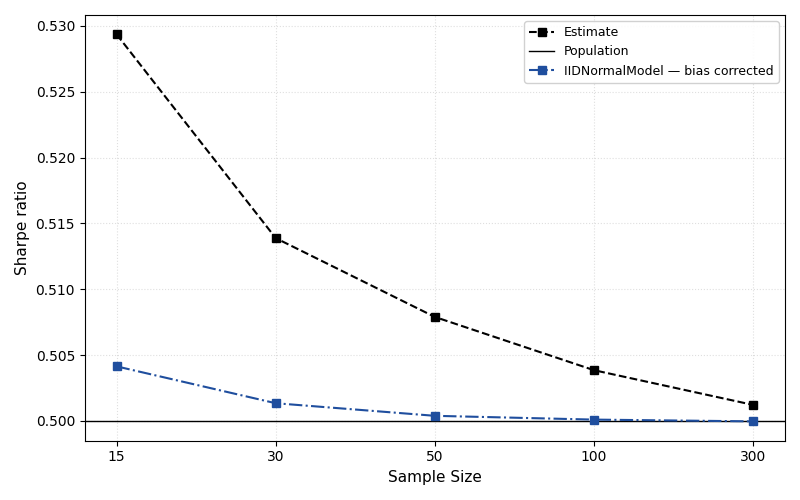
\includegraphics[width=\linewidth,height=1.8cm,keepaspectratio]{figures/iidnormal.png}
      \caption{IID Normal}
    \end{subfigure}\hfill
    \begin{subfigure}{0.31\textwidth}
      \centering
      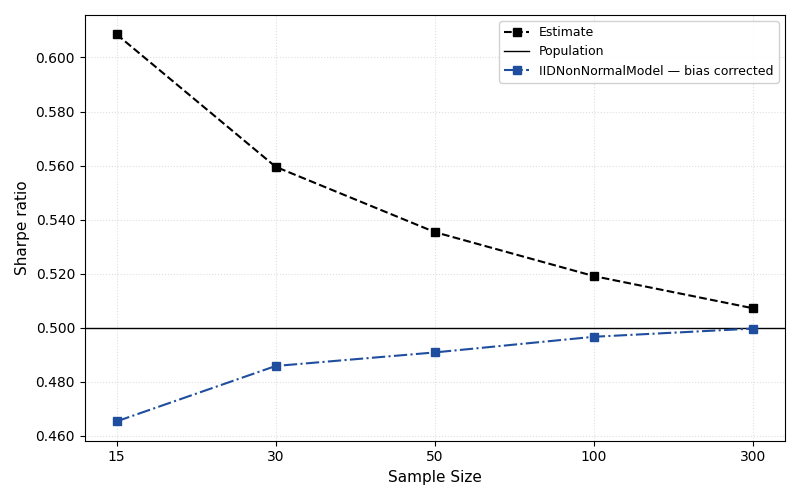
\includegraphics[width=\linewidth,height=1.8cm,keepaspectratio]{figures/iidnonnormal.png}
      \caption{IID Non-Normal}
    \end{subfigure}\hfill
    \begin{subfigure}{0.31\textwidth}
      \centering
      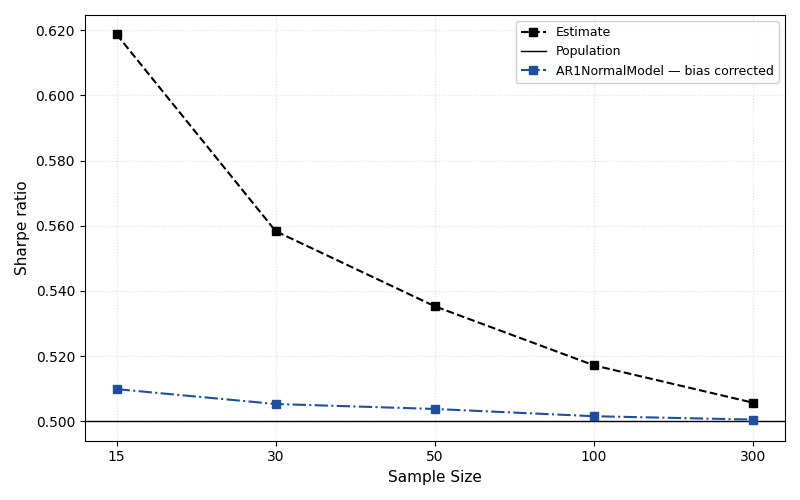
\includegraphics[width=\linewidth,height=1.8cm,keepaspectratio]{figures/arnormal.png}
      \caption{AR(1) Normal}
    \end{subfigure}

    \vspace{0.15em}

    \begin{subfigure}{0.31\textwidth}
      \centering
      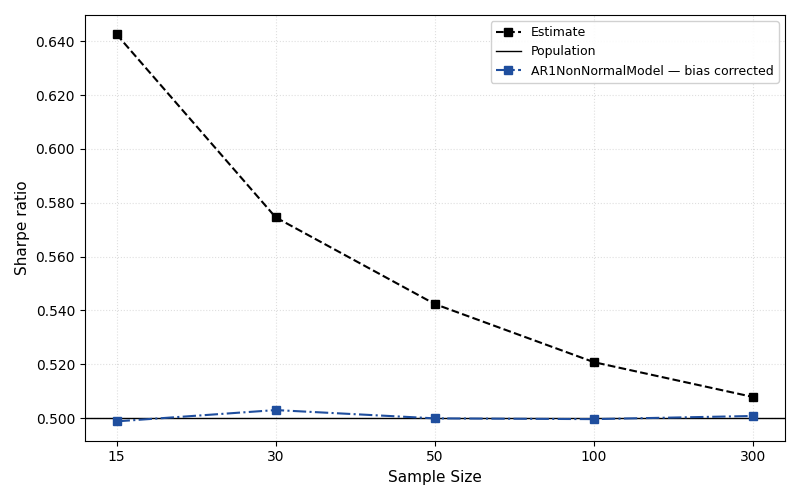
\includegraphics[width=\linewidth,height=1.8cm,keepaspectratio]{figures/arnonnormal.png}
      \caption{AR(1) Non-Normal}
    \end{subfigure}\hfill
    \begin{subfigure}{0.31\textwidth}
      \centering
      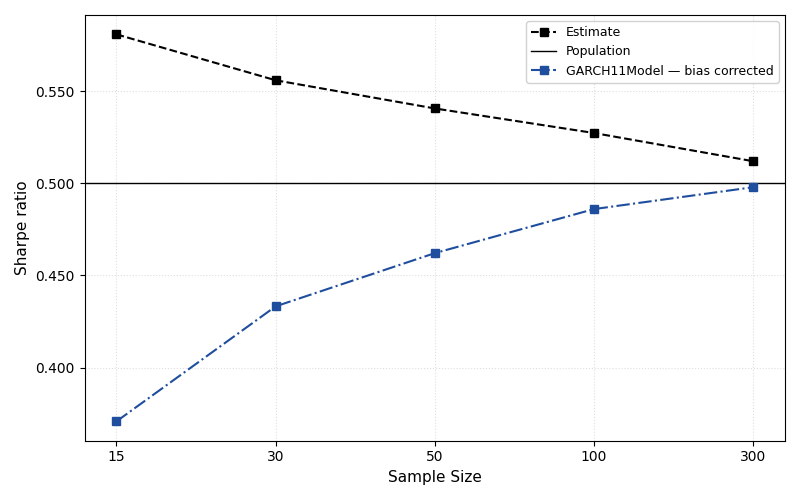
\includegraphics[width=\linewidth,height=1.8cm,keepaspectratio]{figures/garch.png}
      \caption{GARCH(1,1)}
    \end{subfigure}\hfill
    \begin{subfigure}{0.31\textwidth}
      \centering
      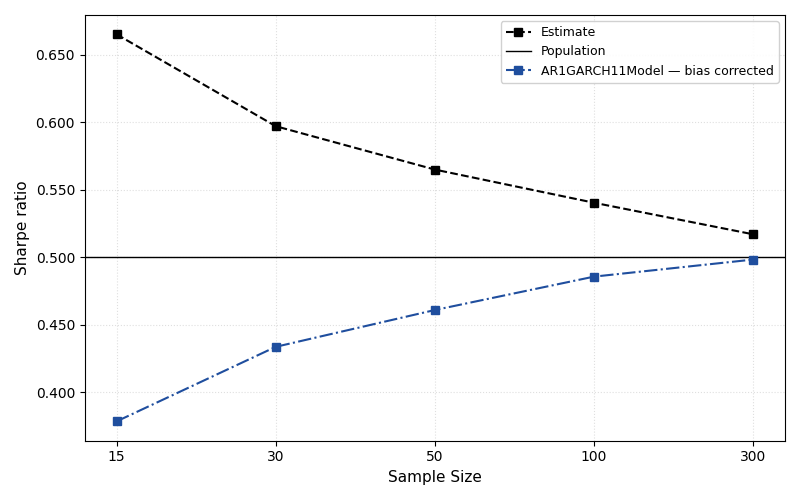
\includegraphics[width=\linewidth,height=1.8cm,keepaspectratio]{figures/argarch.png}
      \caption{AR(1)-GARCH(1,1)}
    \end{subfigure}
    \captionsetup{font=scriptsize,skip=2pt}
    \caption{Individual comparison of the improvement from the bias correction.}
    \label{fig:comp_bias}
  \end{figure}

  \vspace{0.15em}
  {\scriptsize Corrected estimator (blue) converges faster in every model.
  GARCH is slightly off at very small $T$, then overtakes --- reported honestly.}
\end{frame}

%=====================================================================
\section{Does the framework survive real data?}
%=====================================================================

% ---------- SLIDE 12 — ETF data ----------
\begin{frame}{Real data: three SPDR ETFs (2016--2025, weekly)}
  \centering
  \begin{columns}[c]
    \begin{column}{0.5\textwidth}\centering
      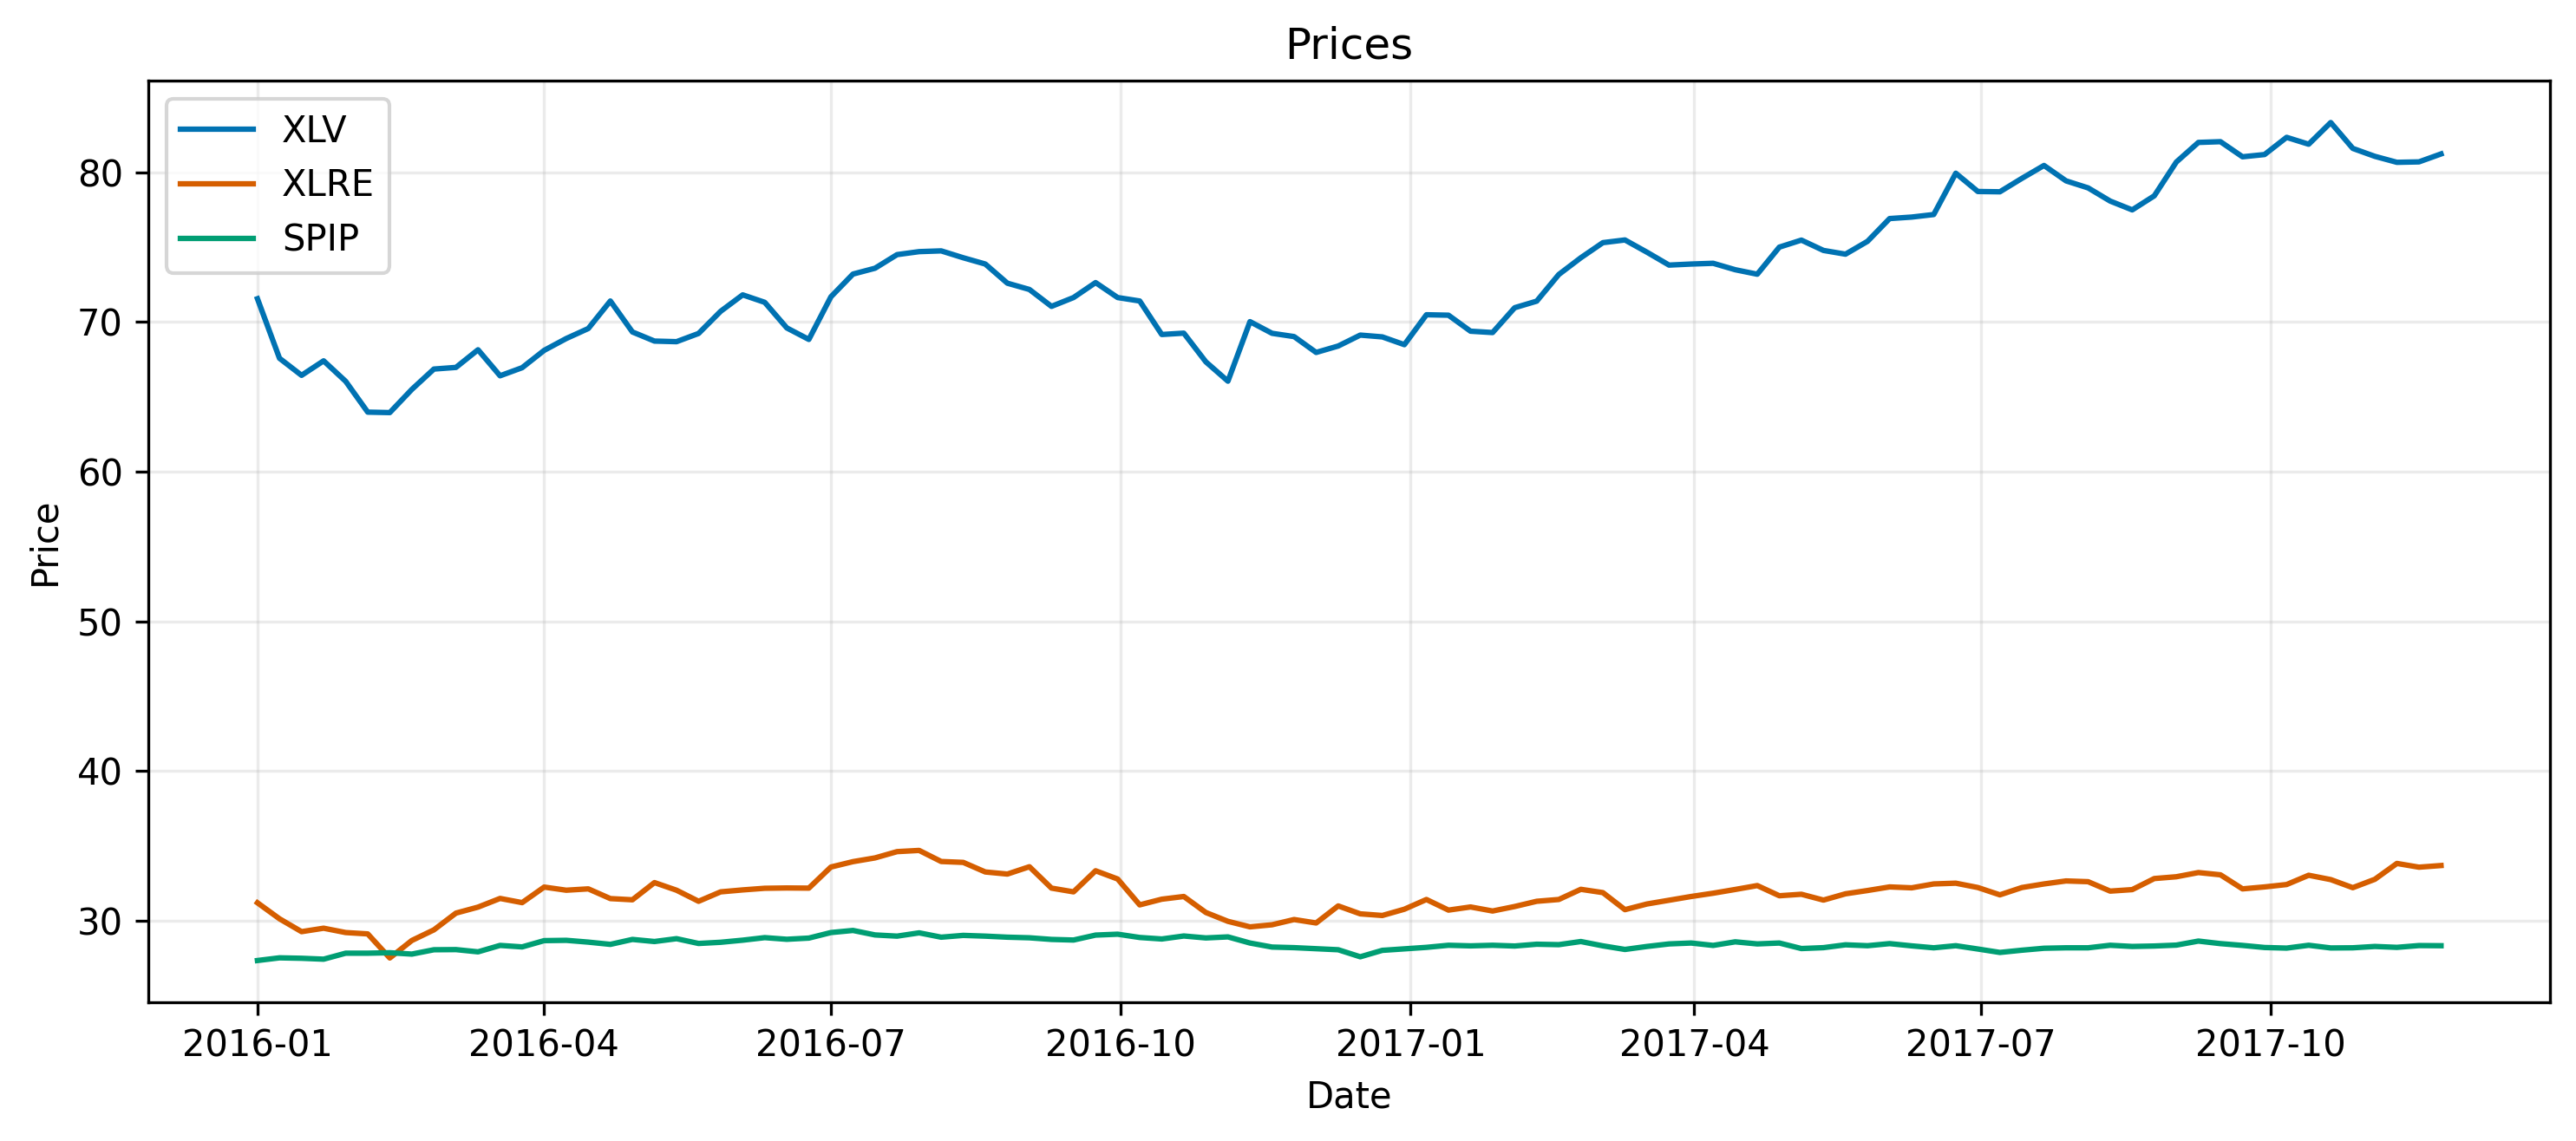
\includegraphics[width=\linewidth,height=3.2cm,keepaspectratio]{figures/prices.png}\\
      {\footnotesize Price levels}
    \end{column}
    \begin{column}{0.5\textwidth}\centering
      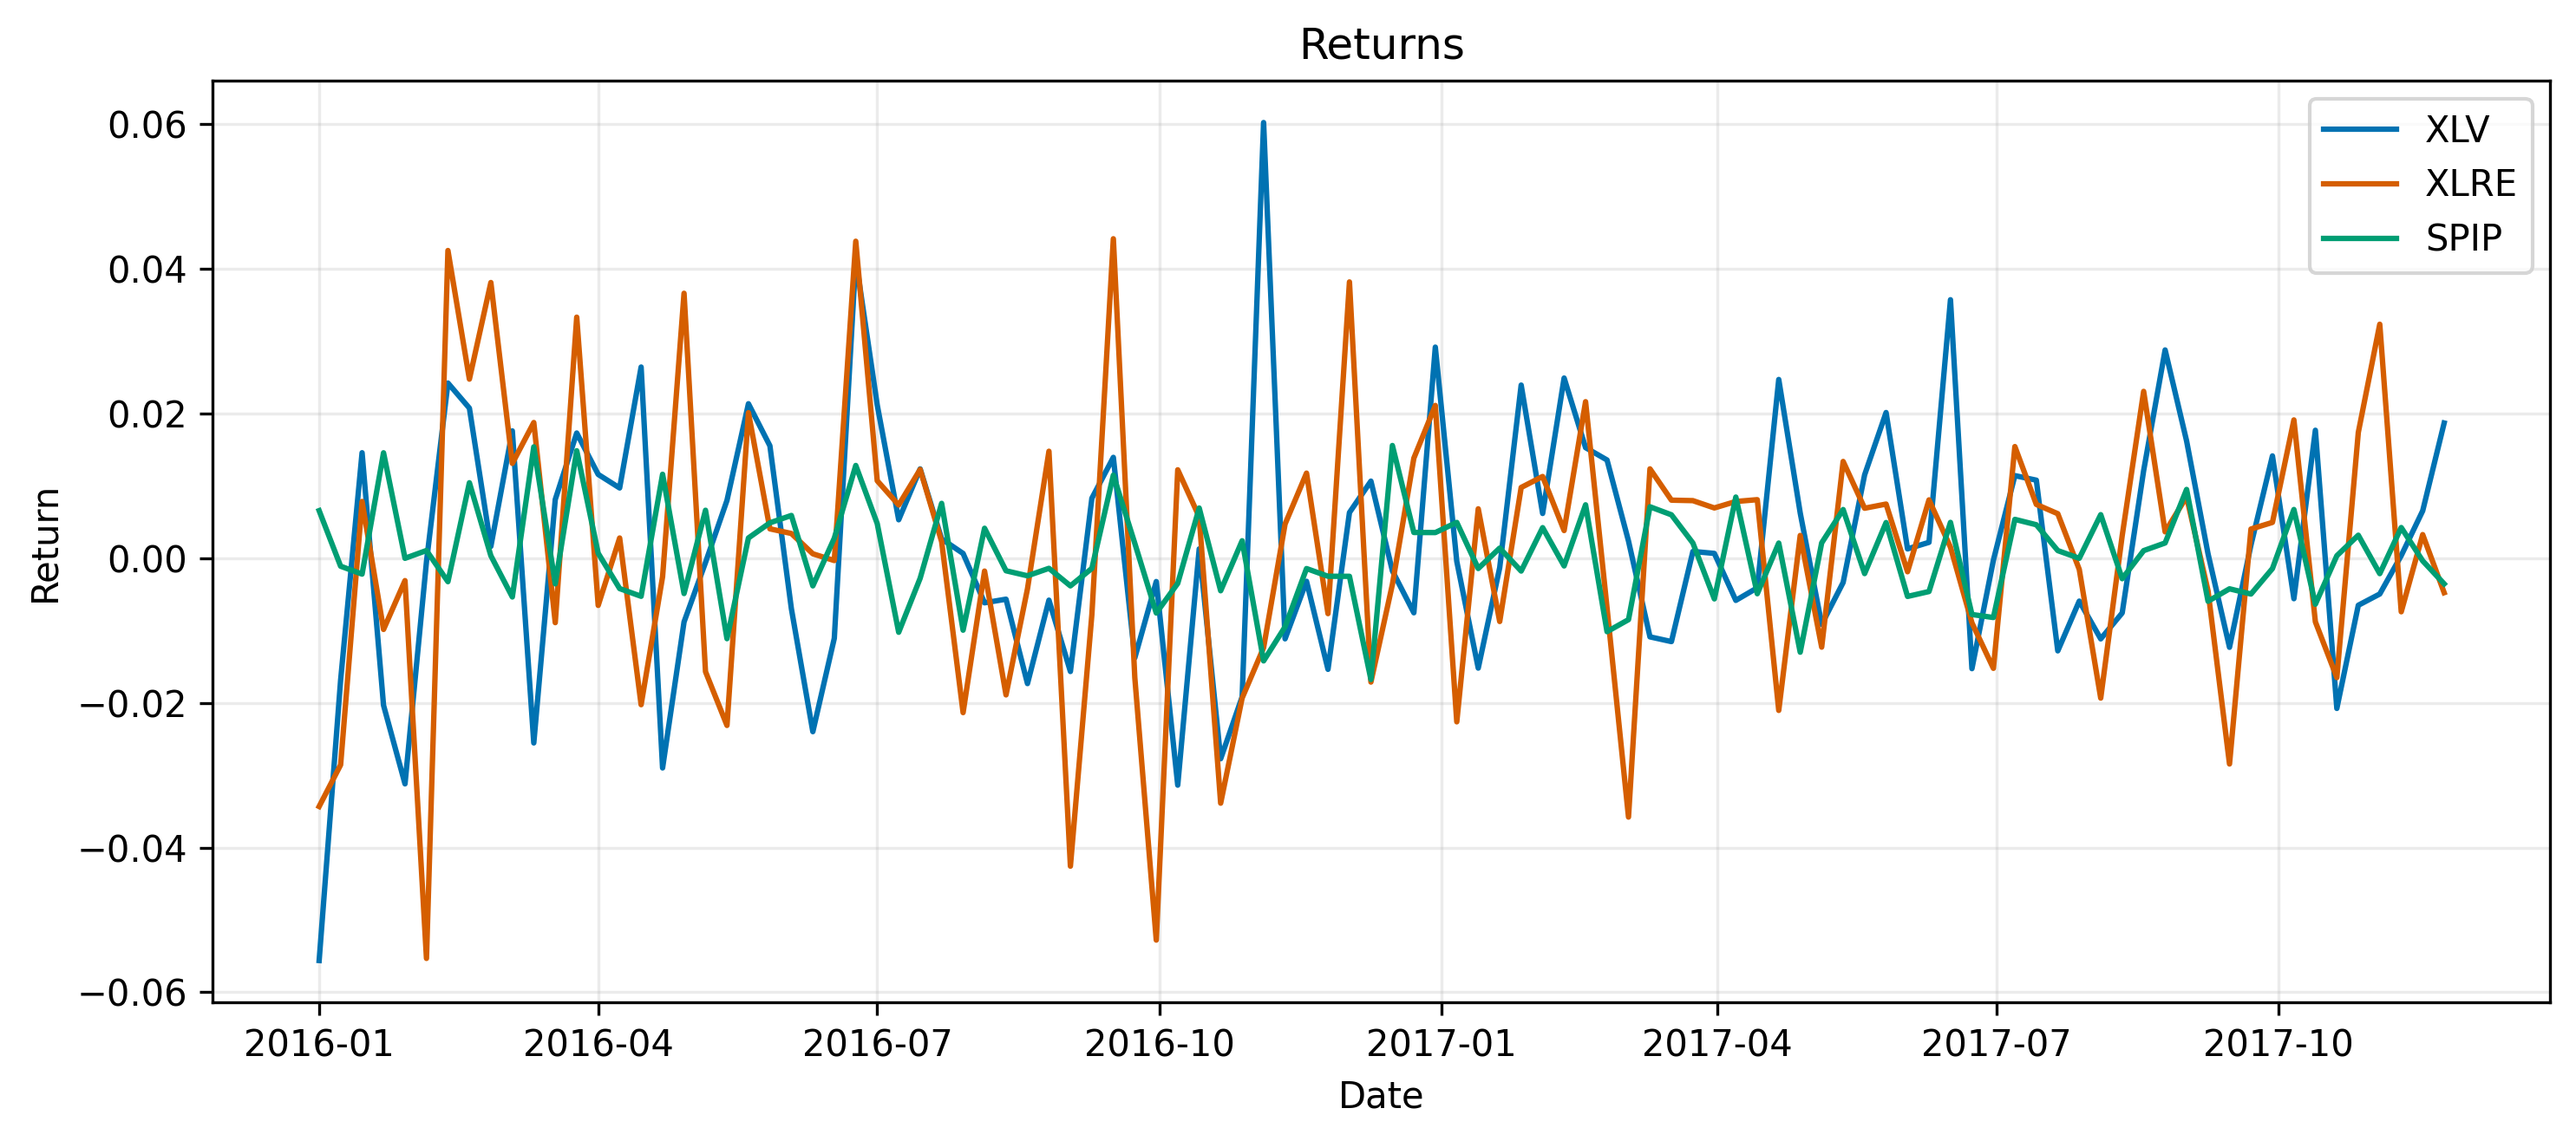
\includegraphics[width=\linewidth,height=3.2cm,keepaspectratio]{figures/returns.png}\\
      {\footnotesize Weekly log-returns}
    \end{column}
  \end{columns}

  \vspace{0.2em}
  {\small Chosen because they show \alert{both} serial correlation in the level
  and conditional heteroskedasticity.}

  \vspace{0.4em}
  \footnotesize
  \begin{tabular}{@{}lcccl@{}}
    \toprule
    Series & Ljung--Box (level) & ARCH-LM & Normality (JB) & Selected specification \\
    \midrule
    XLV  & reject $^{**}$  & reject $^{***}$ & reject $^{***}$ & AR(1)-GARCH(1,1)-skew-$t$ \\
    XLRE & reject $^{***}$ & reject $^{***}$ & reject $^{***}$ & AR(1)-GARCH(1,1)-skew-$t$ \\
    SPIP & reject $^{***}$ & reject $^{***}$ & reject $^{***}$ & AR(1)-GARCH(1,1)-skew-$t$ \\
    \bottomrule
  \end{tabular}

  \normalsize
  \vspace{0.4em}
  {\footnotesize Hierarchical testing (Ljung--Box $\to$ Engle LM $\to$ JB/symmetry)
  selects the same model for all three.}
\end{frame}

% ---------- SLIDE 13 — Probabilistic Sharpe Ratio ----------
\begin{frame}{Inference across models: the Probabilistic Sharpe Ratio}
  \[ \widehat{\mathrm{PSR}}(\mathrm{SR}^\star)
     = \Phi\!\left(\frac{\widehat{\mathrm{SR}} - \mathrm{SR}^\star}
                        {\sqrt{V_{\mathcal{M}}(\hat\theta)/T}}\right),
     \qquad \mathrm{SR}^\star = 0 \]

  {\small Same $\widehat{\mathrm{SR}}$ in every column; only $V_{\mathcal{M}}$ changes.}

  \vspace{0.5em}
  \centering
  \footnotesize
  \begin{tabular}{@{}lcccc@{}}
    \toprule
    Series & iid Normal & AR(1) & GARCH(1,1) & AR(1)-GARCH(1,1) \\
    \midrule
    XLV  & \alert{95.80} & 96.95 & 94.94 & \alert{96.22} \\
    XLRE & 76.51         & 79.89 & 76.14 & 78.72 \\
    SPIP & 42.88         & 42.20 & 42.80 & 42.21 \\
    \bottomrule
  \end{tabular}

  \normalsize
  \vspace{0.4em}
  {\small XLV crosses the 95\% line; the correction is \textbf{non-monotone}
  in model complexity.}

  \vspace{0.3em}
  {\scriptsize Comparing PSRs across columns is not a formal model test --- each uses a
  different reference distribution. It mirrors an analyst committing to one specification.}
\end{frame}

%=====================================================================
\section{Beyond a single number: pairing with VaR}
%=====================================================================

% ---------- SLIDE 14 — Joint distribution with VaR ----------
\begin{frame}{Beyond one metric: joint distribution with Value-at-Risk}
  \[ \sqrt{T}\,
   \begin{pmatrix} \widehat{\mathrm{SR}}-\mathrm{SR} \\[3pt]
                   \widehat{\mathrm{VaR}}-\mathrm{VaR} \end{pmatrix}
   \;\xrightarrow{\,d\,}\;
   \mathcal{N}\!\left(\begin{pmatrix} 0 \\[3pt] 0 \end{pmatrix},\; V_{h}\right) \]

  \vspace{0.3em}
  \begin{columns}[c]
    \begin{column}{0.5\textwidth}\centering
      {\footnotesize Non-parametric (empirical quantile)}
      \[ V^{np}_{h} = \begin{pmatrix}
         1+\tfrac{\mathrm{SR}^2}{2} & \tfrac{\mu z_\alpha}{2}-\sigma \\[6pt]
         \tfrac{\mu z_\alpha}{2}-\sigma & \sigma^2\,\dfrac{\alpha(1-\alpha)}{\varphi(z_\alpha)^2}
         \end{pmatrix} \]
    \end{column}
    \begin{column}{0.5\textwidth}\centering
      {\footnotesize Parametric (Gaussian)}
      \[ V^{p}_{h} = \begin{pmatrix}
         1+\tfrac{\mathrm{SR}^2}{2} & \tfrac{\mu z_\alpha}{2}-\sigma \\[6pt]
         \tfrac{\mu z_\alpha}{2}-\sigma & \sigma^2\Bigl(1+\tfrac{z_\alpha^2}{2}\Bigr)
         \end{pmatrix} \]
    \end{column}
  \end{columns}

  \vfill
  \begin{columns}[T]
    \begin{column}{0.62\textwidth}
      \begin{itemize}\small
        \item \alert{Negative covariance} ($\tfrac{\mu z_\alpha}{2}-\sigma<0$):
              a shock that raises $\widehat{\mathrm{SR}}$ also lowers $\widehat{\mathrm{VaR}}$
              --- they err together.
        \item \alert{Only the $(2,2)$ entry differs.} Parametric is more efficient;
              the gap grows in the tail.
      \end{itemize}
    \end{column}
    \begin{column}{0.38\textwidth}\centering
      \scriptsize
      \begin{tabular}{@{}lccc@{}}
        \toprule
        $\alpha$ & $0.05$ & $0.01$ & $0.001$ \\
        \midrule
        $V^{np}_{22}/V^{p}_{22}$ & $\approx 1.90$ & $\approx 3.77$ & $\approx \alert{11}$ \\
        \bottomrule
      \end{tabular}
    \end{column}
  \end{columns}
  {\scriptsize \quad $\varphi(\cdot)$ = standard normal density,\; $z_\alpha=\Phi^{-1}(\alpha)$.}
\end{frame}

% ---------- SLIDE 15 — Efficiency vs robustness ----------
\begin{frame}{Efficiency vs robustness, in one picture}
  \begin{columns}[T]
    \begin{column}{0.5\textwidth}\centering
      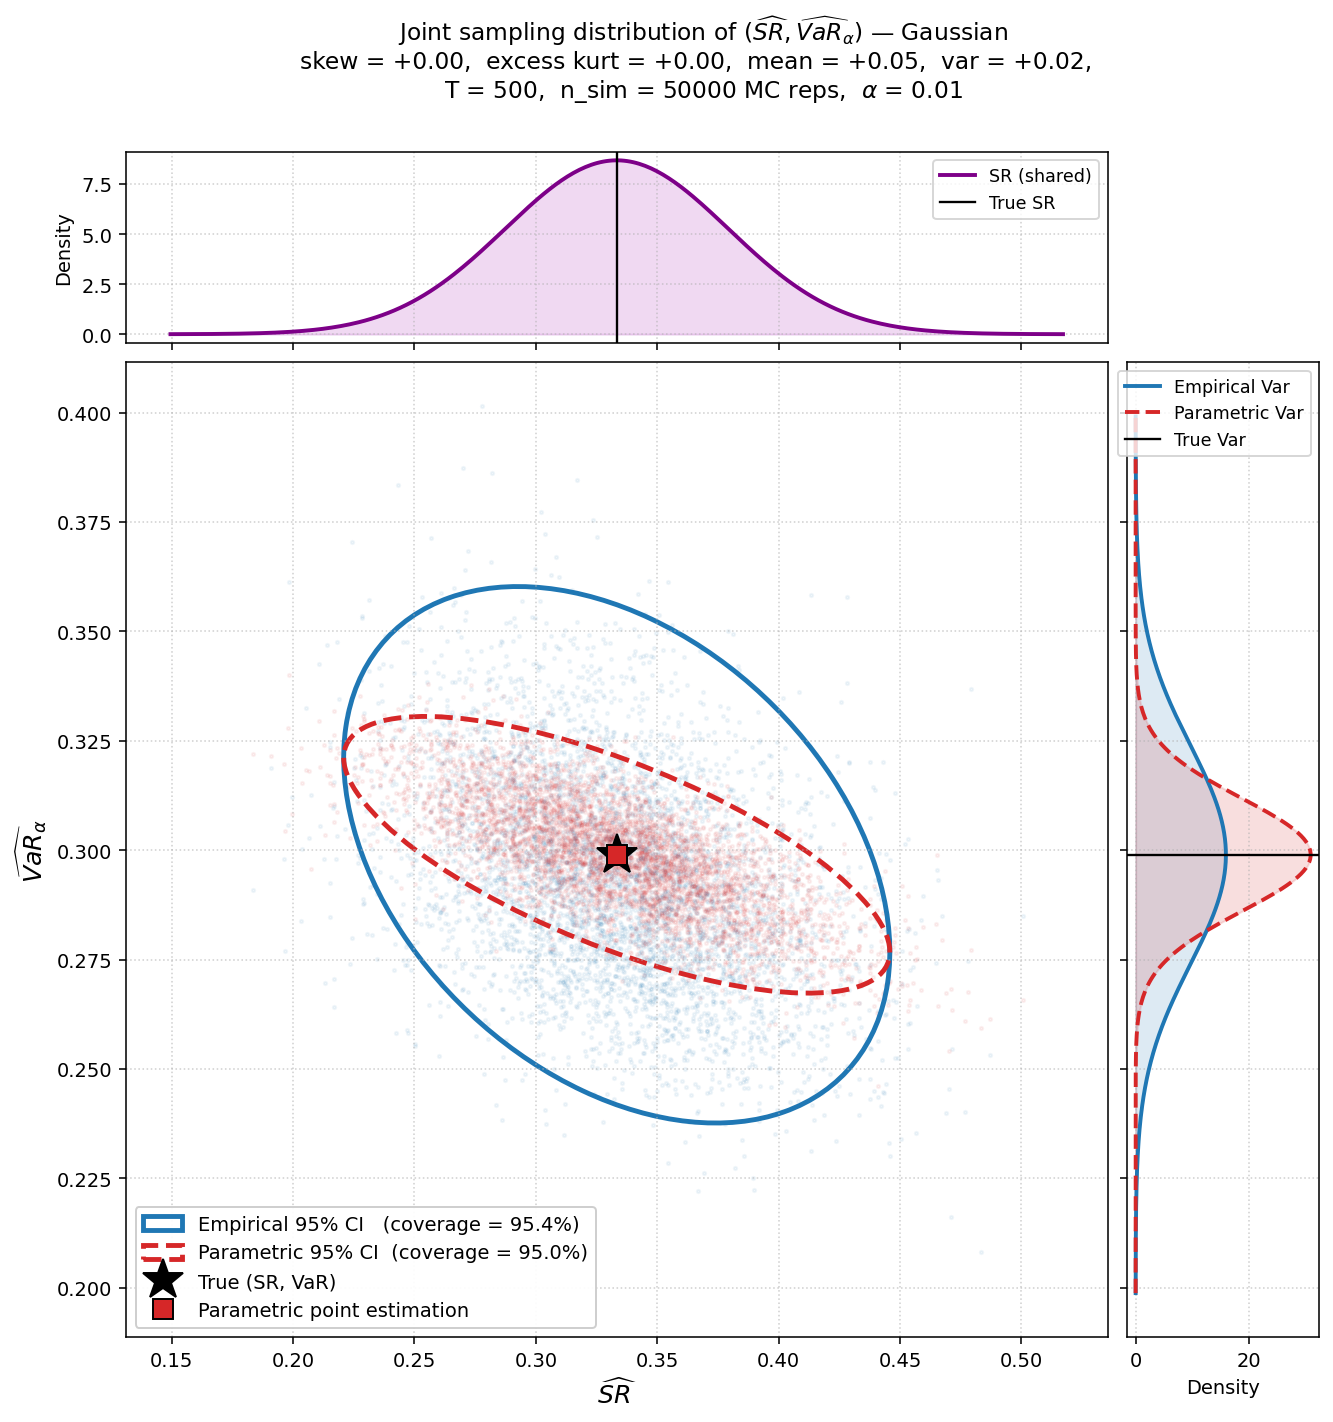
\includegraphics[width=\linewidth,height=4.6cm,keepaspectratio]{figures/sr_var_gaussian.png}\\
      {\footnotesize Gaussian returns: parametric ellipse \textbf{inside}
      the non-parametric one. Coverage 95.0\% vs 95.4\%.}
    \end{column}
    \begin{column}{0.5\textwidth}\centering
      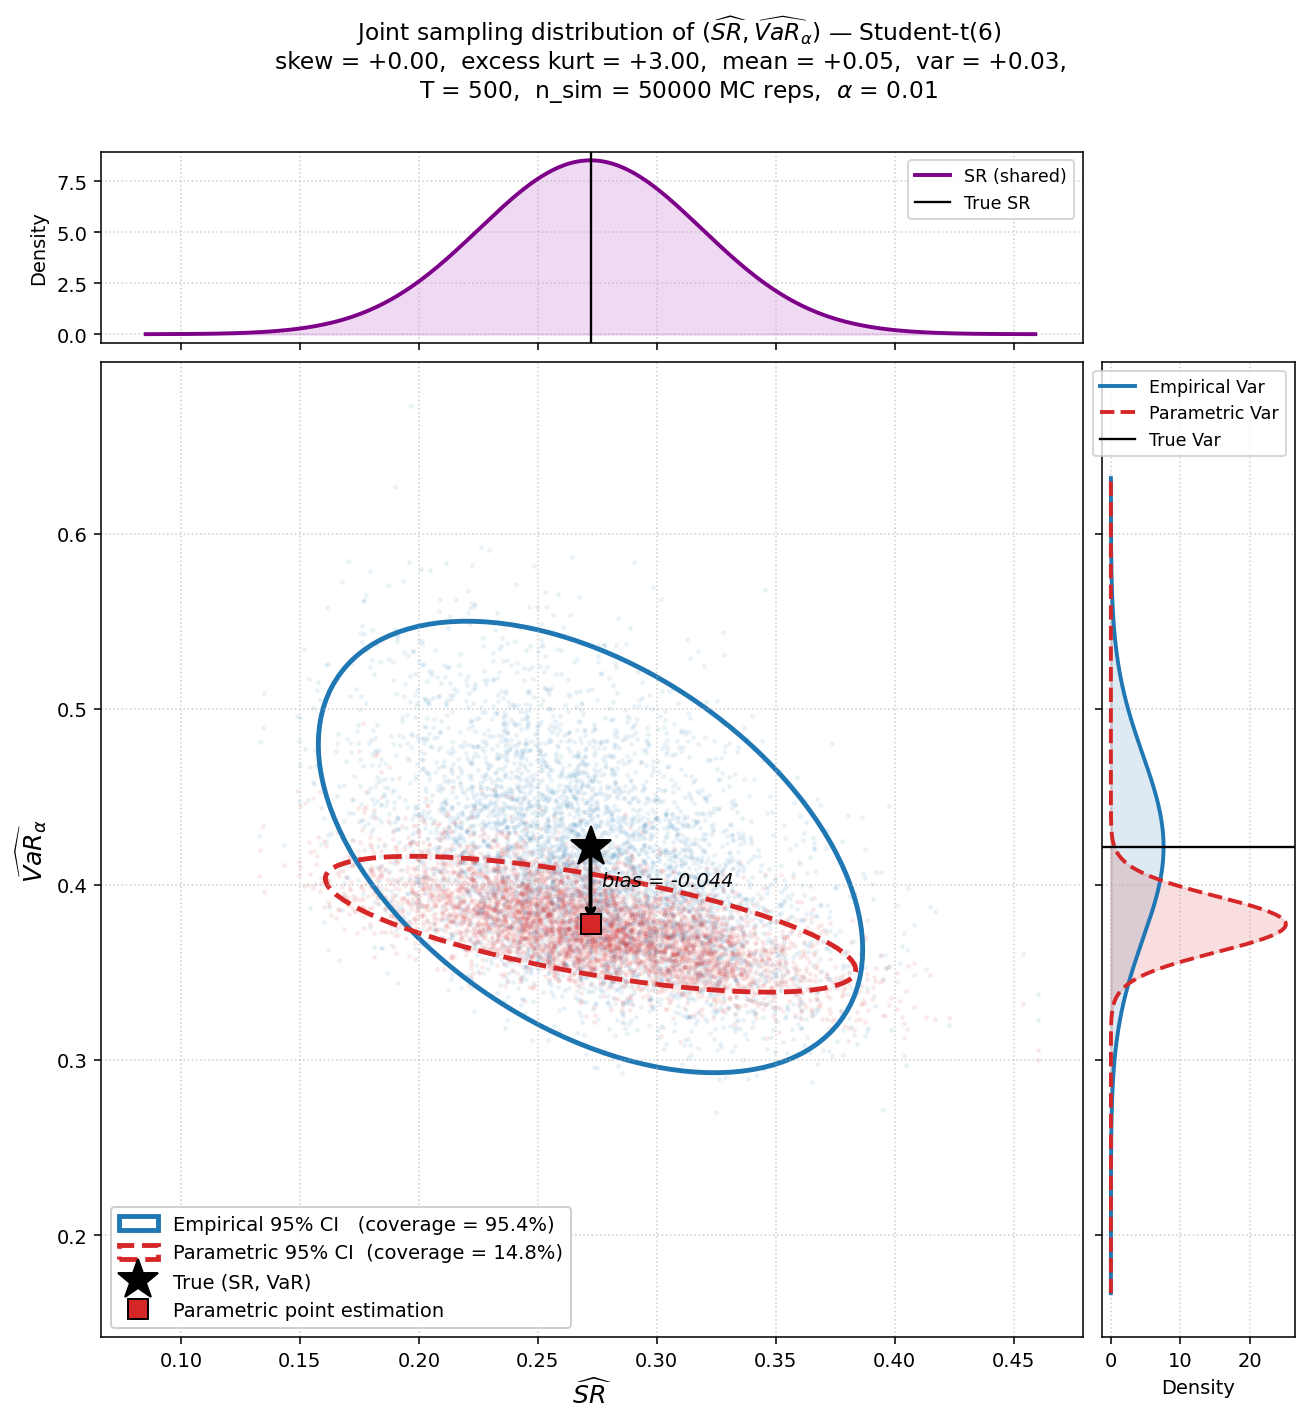
\includegraphics[width=\linewidth,height=4.6cm,keepaspectratio]{figures/sr_var_student_t(6).png}\\
      {\footnotesize Student-$t_6$ returns: parametric ellipse \alert{biased}
      (shift $-0.044$), coverage \alert{14.8\%}; non-parametric stays \alert{95.4\%}.}
    \end{column}
  \end{columns}
  \vspace{0.4em}
  \begin{center}
  Parametric wins when the distribution is right; fails badly when it is wrong.
  \end{center}
\end{frame}

% ---------- SLIDE 16 — Closing ----------
\begin{frame}{How reliable is this number?}
  \begin{enumerate}
    \item \textbf{Precision} depends on the model assumed for returns.
    \item The \textbf{wrong model} makes intervals lie --- usually too narrow.
    \item In \textbf{small samples} the estimate is biased --- the popular fix is too small.
    \item Even when \textbf{correctly specified}, parameters near the \textbf{boundaries}
          ($\phi$, $\alpha+\beta$ persistence) cause trouble.
  \end{enumerate}

  \vspace{0.6em}
  \begin{center}
  {\large A single framework --- built on the long-run variance matrix $S$ ---\\
   answers all four for the AR-GARCH world real returns live in.}
  \end{center}

  \vfill
  {\footnotesize Thank you --- questions welcome.\hfill
   Code: \texttt{github.com/Fabro2701/sharpe\_ratio\_TFM}}
\end{frame}

\end{document}